% Chapter 4

\chapter{Image Processing} % Main chapter title

\label{Chapter4} % For referencing the chapter elsewhere, use \ref{Chapter4} 

\lhead{Chapter 4. \emph{Image Processing}} % This is for the header on each page - perhaps a shortened title

%----------------------------------------------------------------------------------------

%----------------------------------------------------------------------------------------
\begin{figure}[h]
        \centering
        \begin{subfigure}[b]{0.5\textwidth}
                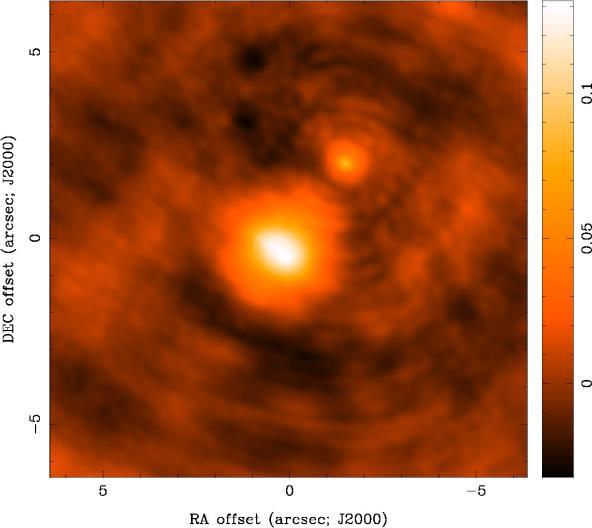
\includegraphics[width=\textwidth]{Figures/dirty}
                \caption{An initial dirty map}
                \label{fig:noWeightDirty}
        \end{subfigure}%
        ~ %add desired spacing between images, e. g. ~, \quad, \qquad, \hfill etc.
          %(or a blank line to force the subfigure onto a new line)
        \begin{subfigure}[b]{0.5\textwidth}
                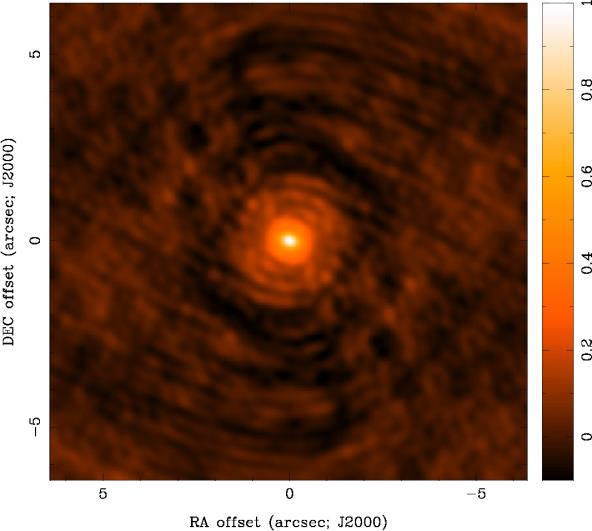
\includegraphics[width=\textwidth]{Figures/scaledbeam}
                \caption{The weighted dirty map}
                \label{fig:weightDirty}
        \end{subfigure}
        \caption[The end result of image reconstruction]{The end result of image reconstruction~\citep[Slide 51]{wilner.siw2014}}\label{fig:imageReconstruction}
\label{fig:Dirty}
\end{figure}
\section{Introduction - Image Processing}\
\label{sec:about4}
Images obtained from the visibility, $V(u,v)$, corresponding to the antenna responses to the signals from the sky are somehow defective and known as “dirty images” see Fig.~\ref{fig:Dirty}.  In order to obtain the highest dynamic range in radio images, both good spatial frequency coverage and effective image processing are required~(\citet[Pg.~426]{thompson2008interferometry}).

Let’s first relate to the principal deficiencies limiting the accuracy of the synthesised images. These are the limited distribution of spatial frequencies in the $(u,v)$ plane and errors in the measurements themselves. One way to improve on the limited spatial frequency coverage is by deconvolution processes that allow the unmeasured visibility to take nonzero values within some general constraints in the image. While the errors in the measurements themselves can be refined by calibrating the measured visibilities $V’(u,v)$ in order to approximate the true visibilities $V(u,v)$ as closely as possible~(\citet[Pg.~426]{thompson2008interferometry}) which was discussed in chapter~\ref{Chapter3}.

\begin{equation}
I_0(l,m) = I(l,m)\ast{\ast}{\,}b_0(l,m)
\end{equation}

$I_0(l,m)$: measured intensity distribution\\
$I(l,m)$: true intensity\\
$b_0(l,m)$: synthesized beam\\

The measured intensity distribution, $I_0(l,m)$, obtained in synthesis mapping can be regarded as the true intensity, $I(l,m)$, convolved with the synthesized beam, $b_0(l,m)$, illustrated there. The double asterisk indicates two-dimensional convolution.\\
Knowing the measured intensity distribution and the synthesized beam we might want to solve for the true intensity by an analytical procedure for deconvolving two functions that is achieved by taking the Fourier Transform of the convolution, which is equal to the product of the Fourier transforms of the components, dividing out the Fourier transform of the known function, and transforming back~\citep[Pg.~426]{thompson2008interferometry}. 

\begin{equation}
\label{eq:convolBack}
I_0(l,m) \rightleftharpoons [V(u,v)[W(u,v)w_u(u,v)w_t(u,v)]
\end{equation}

$V(u,v)$: visibility function\\
$W(u,v)$: spatial transfer function\\
$w_u(u,v)$: weighting required to obtain effective uniform density of data in the $(u,v)$ plane.\\
$w_t(u,v)$: applied taper\\

However, the transfer function contains areas where it is zero, so we cannot just divide it out to obtain the visibility function. The holes, that are values at which visibilities are not measured, present a fundamental problem, and any procedure aiming at improving the true intensity other than weighting of the visibility must involve placing nonzero visibility values in the unmeasured $(u, v)$ areas. Therefore as pointed out by Bracewell and Roberts in 1954 there can be an infinite number of solutions to the above convolution, since one can add any arbitrary visibility values in the unsampled areas of the $(u,v)$ plane. The Fourier transform of these added values constitutes an invisible distribution that cannot be detected by any instrument with corresponding zero areas in the transfer function~\citep[Pg.~427]{thompson2008interferometry}.

It may thus be argued that in interpreting observations from any radio telescope, one should maintain only zeros in the unmeasured regions of spectral sensitivity, to avoid arbitrarily generating information. Alas, zeros are themselves arbitrary values some of which are certainly wrong. What we want is a procedure that allows the visibility at the unmeasured points to take values consistent with the most reasonable or likely intensity distribution, while minimizing the addition of arbitrary detail~\citep[Pg.~427]{thompson2008interferometry}.

Characteristics such as positivity of intensity and confinement of the angular structure of a source are expected and they can be introduced into the imaging process. Instrumental artifacts such as negative intensity values and extensive sinusoidal structure are to be removed~\citep[Pg.~427]{thompson2008interferometry}.
\section{Deconvolution Procedures}
\label{sec:deconvTech}
Processes for the removal of effects of sidelobes or defects in the dirty images are in fact deconvolution procedures.
There exists different methods such as the CLEAN algorithm, MEM standing for Maximum Entropy Method, NNLS for non-negative, least squares algorithm for this report we'll focus on the CLEAN algorithm{~\citep[for~the~others~see][Sec.~10.3]{thompson2008interferometry}}.
\subsection{The CLEAN algorithm}
\label{sec:cleanAlgo}
~\citep[From Pgs.~427-429]{thompson2008interferometry}
The CLEAN algorithm is one of the most successful deconvolution procedures devised by Högbom in 1974. It is basically a numerical deconvolving process applied in the $(l,m)$ domain. It involves breaking down of the intensity distribution into point-source responses and then replacing each one with the corresponding response to a “clean” beam, that is, a beam free of sidelobes, particularly negative ones, and that its Fourier transform should be constant inside the sampled region of the $(u ,v)$ plane and rapidly fall to a low level outside it. However these characteristics are essentially incompatible since a sharp cutoff in the $(u, v)$ plane results in oscillations in the $(l,m)$ plane.

Here are the principal steps to follow :

Firstly, we compute the map and the response to a point source by Fourier transformation of the visibility and the weighted transfer function. We refer the functions, synthesised intensity and synthesised beam as the “dirty map” and the “dirty beam,” respectively. We must also ensure that the spacing of the sample points in the $(l,m)$ plane does not exceed about one-third of the synthesised beamwidth.
We then find the highest intensity point on the map and subtract the response to a point source, including the full sidelobe pattern, centered on that position assuming that each dirty-beam response subtracted represents the response to a point source. The visibility function of which is a pair of real and imaginary sinusoidal corrugations that extend to infinity in the $(u,v)$ plane. The peak amplitude of the subtracted point source is equal to $\gamma$ times the corresponding map amplitude where,  $\gamma$, is the loop gain, by analogy with negative feedback in electrical systems, and commonly has a value of a few tenths. We record the position and amplitude of the component that is removed by inserting a delta-function component into a model that will become the cleaned map.
This process is then repeated iteratively until all significant source structure has been removed from the map. There are several possible indicators of this condition for example, one can compare the highest peak with the rms level of the residual intensity, look for the first time that the rms level fails to decrease when a subtraction is made, or note when significant numbers of negative components start to be removed.
These 3 steps can be represented by a model intensity distribution consisting of a series of delta functions with magnitudes and positions representing the subtracted components. Since the modulus of the Fourier transform of each delta function extends uniformly to infinity in the $(u,v)$ plane, the visibility is extrapolated as required
beyond the cutoff of the transfer function.

As delta-function components do not constitute a satisfactory model for astronomical purposes. Groups of delta functions with separations no greater than the beamwidth may actually represent extended structure. So as a fourth step, we convolve the delta functions in the cleaned model with a clean-beam response, that is, we replace each delta function with a clean-beam function of corresponding amplitude. The clean beam is often chosen to be a Gaussian with a half-amplitude width equal to that of the original synthesised (dirty) beam, or some similar function that is free from negative values. A Gaussian beam is preferred as it introduces a Gaussian taper in the $(u,v)$ plane which tapers the measured data and the unmeasured data generated by CLEAN and the resulting intensity distribution no longer agrees with the measured visibility data. However, the absence of large, near-in sidelobes improves the dynamic range of the image, that is, it increases the range of intensity over which the structure of the image can reliably be measured. This thereby also removes the danger of over-interpretation. At the point that the component subtraction is stopped, it is generally assumed that the residual intensity distribution consists mainly of the noise. Retaining the residual distribution within the map is, like the convolution with the clean beam, a non ideal procedure that is necessary to prevent misinterpretation of the final result. Finally, we add the residual intensities obtained above into the clean-beam map, which is the output of the process. If we did not add the residuals, there would be an amplitude cut-off in the structure corresponding to the lowest subtracted component. Also, the presence of the background fluctuations provides an indication of the level of uncertainty in the intensity values.

Any intensity feature for which the visibility function is the same within the $(u,v)$ area sampled by the transfer function would produce a response in the map identical to the point source response. CLEAN was initially developed on the basis of the situation pointed out by Högbom that much of the sky is a random distribution of point sources on an empty background. It can also be regarded as an interpolation in the $(u,v)$ plane. Nevertheless, experience shows that CLEAN also works on extended and complicated sources.
 
The issue we discussed above about this equation~\ref{eq:convolBack} which was that we cannot directly divide out the weighted transfer function on the right-hand side of equation because it is truncated to zero outside the areas of measurement. In CLEAN, this problem is solved by analysing the measured visibility into sinusoidal visibility components and then removing the truncation so that they extend over the full $(u,v)$ plane. Selecting the highest peak in the $(l, m )$ plane is equivalent to selecting the largest complex sinusoid in the $(u,v)$ plane.

Here following in figures~\ref{fig:CLEANed} is an example of the effect of processing with the CLEAN algorithm.%
\begin{figure}
        \centering
        \begin{subfigure}[b]{\textwidth}
        \centering
                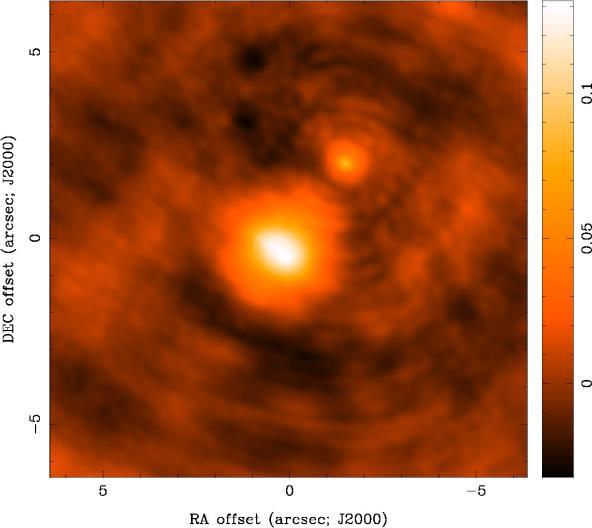
\includegraphics[scale=0.6]{Figures/uv-coverage/cleanD1}
                \caption{Dirty map}
                \label{fig:dirtycl}        
        \end{subfigure}% 
        
        ~ %add desired spacing between images, e. g. ~, \quad, \qquad, \hfill etc.
          %(or a blank line to force the subfigure onto a new line)
        \begin{subfigure}[b]{0.5\textwidth}
			\centering
                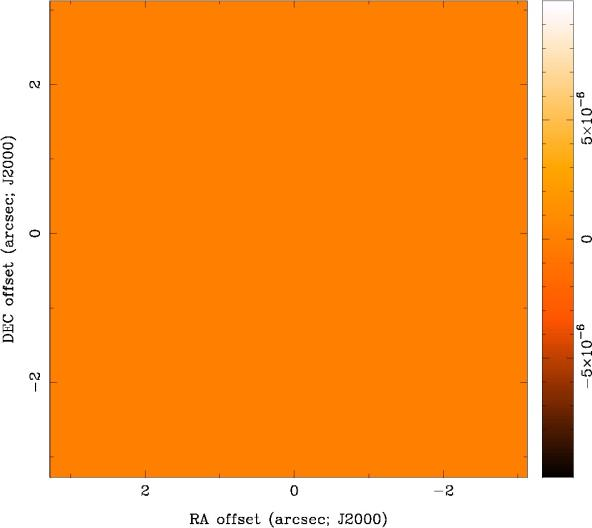
\includegraphics[scale=0.6]{Figures/uv-coverage/cleanD1map}
                \caption{0 Clean components}
                \label{fig:clmap1}
        \end{subfigure}%
       %
        \begin{subfigure}[b]{0.5\textwidth}
		\centering                
                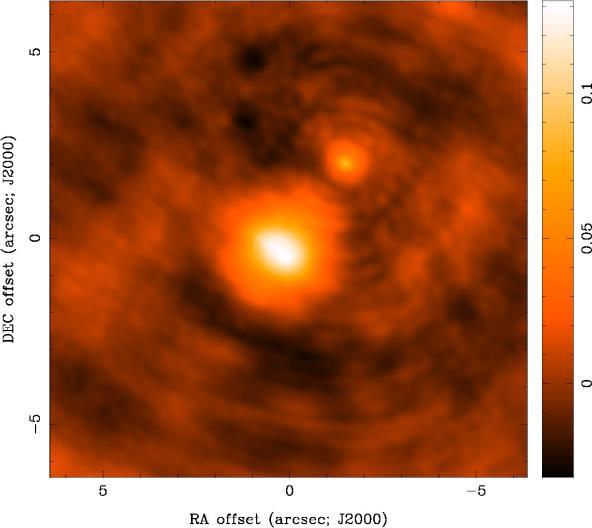
\includegraphics[scale=0.6]{Figures/uv-coverage/cleanD1res}
                \caption{Residual Map}
                \label{fig:ResMap1}
        \end{subfigure} %
        ~ %add desired spacing between images, e. g. ~, \quad, \qquad, \hfill etc.
          %(or a blank line to force the subfigure onto a new line)
        \begin{subfigure}[b]{0.5\textwidth}
		\centering                
                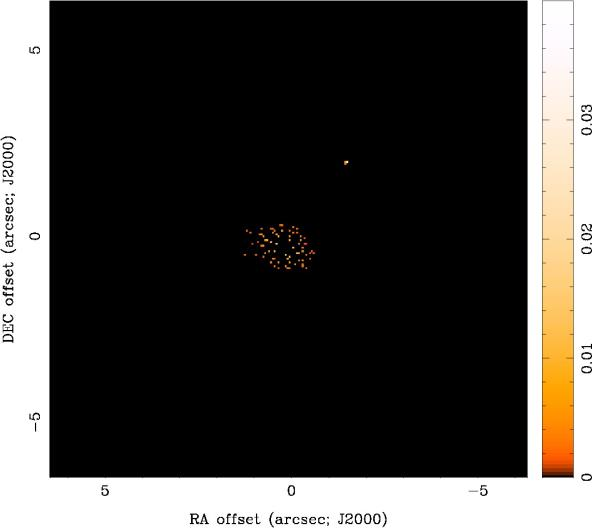
\includegraphics[scale=0.6]{Figures/uv-coverage/cleanD100map}
                \caption{100 Clean components}
                \label{fig:clmap100}
        \end{subfigure}%
          \begin{subfigure}[b]{0.5\textwidth}
				\centering                
                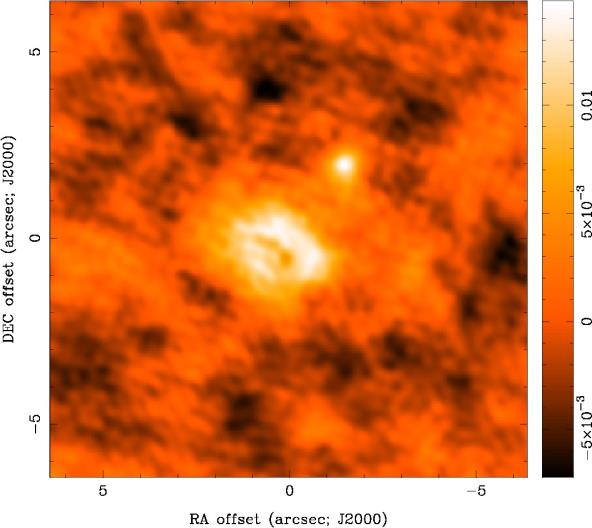
\includegraphics[scale=0.6]{Figures/uv-coverage/cleanD100res}
                \caption{Residual Map}
                \label{fig:ResMap100}
        \end{subfigure} %
        ~ %add desired spacing between images, e. g. ~, \quad, \qquad, \hfill etc.
          %(or a blank line to force the subfigure onto a new line)
        \begin{subfigure}[b]{0.5\textwidth}
				\centering                
                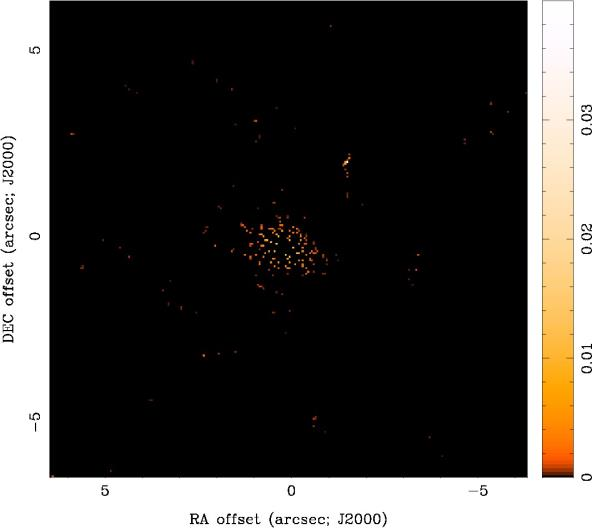
\includegraphics[scale=0.6]{Figures/uv-coverage/cleanD583map}
                \caption{583 Clean components }
                \label{fig:clmap583}
        \end{subfigure}%
        \begin{subfigure}[b]{0.5\textwidth}
				\centering                
                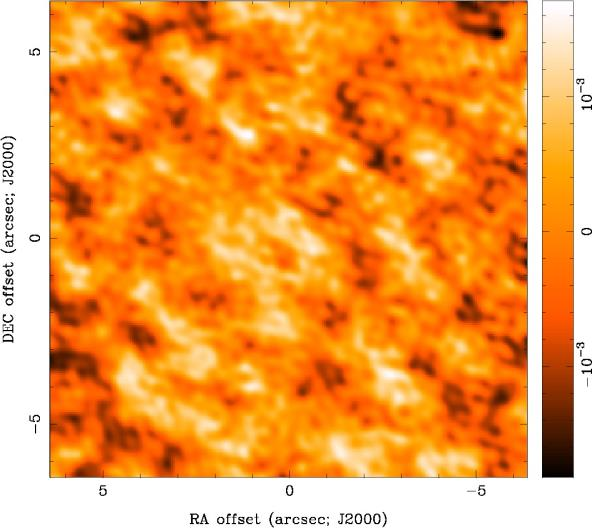
\includegraphics[scale=0.6]{Figures/uv-coverage/cleanD583res}
                \caption{Residual Map}
                \label{fig:ResMap583}
        \end{subfigure} %%
        ~ %add desired spacing between images, e. g. ~, \quad, \qquad, \hfill etc.
          %(or a blank line to force the subfigure onto a new line)
        \begin{subfigure}[b]{0.5\textwidth}
        \centering
                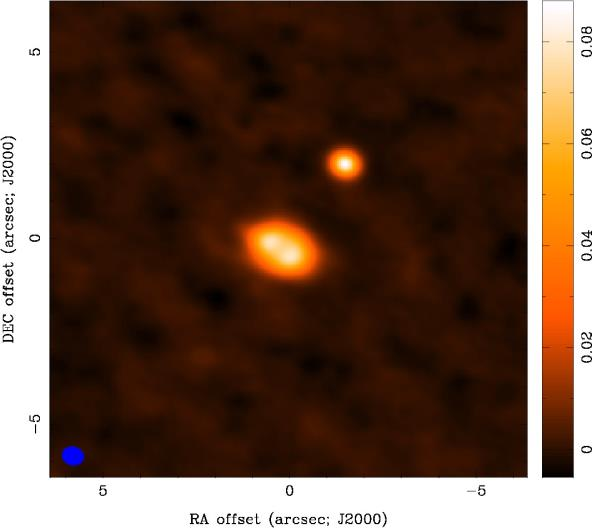
\includegraphics[scale=0.7]{Figures/uv-coverage/cleanRes}
                \caption{CLEANed Map}
                \label{fig:Restmap}
        \end{subfigure}%%
        \caption[CLEAN process]{ CLEAN process ~\citep[Slide 54,56,58,59]{wilner.siw2014}}\label{fig:CLEANed}
\end{figure}
\newpage
\subsection{Performance of the CLEAN algorithm}
\label{sec:cleanPerf}
~\citep[From Pgs.~429-432]{thompson2008interferometry}
As a procedure for removing sidelobe responses, CLEAN is easy to understand. Being highly nonlinear, however, CLEAN does not yield readily to a complete mathematical analysis. Some conclusions have been derived by Schwarz in 1978, who has shown that conditions for convergence of CLEAN are that the synthesised beam must be symmetrical and its Fourier transform, that is, the weighted transfer function, must be non-negative. These conditions are fulfilled in the usual synthesis procedure. Schwarz’s analysis also indicates that if the number of delta-function components in the CLEAN model does not exceed the number of independent visibility data, CLEAN converges to a solution that is the least-squares fit of the Fourier transforms of the delta-function components to the measured visibility. In enumerating the visibility data, either the real and imaginary parts or the conjugate values (but not both) are counted independently. In maps made using the FFT algorithm there are equal numbers of grid points in the $(u,v$) and $(l, m)$ planes, but not all $(u,v)$ grid points contain visibility measurements. To maintain the condition for convergence it is a common procedure to
apply CLEAN only within a limited area, of the original map.

In order to clean a map of a given dimension, it is necessary to have a beam pattern of twice the map dimensions so that a point source can be subtracted from any location in the map. However, it is often convenient for the map and beam to be the same size. In this case only the central quarter of the map can be properly processed. Thus, it is commonly recommended that the map obtained from the initial Fourier transform should have twice the dimensions required for the final map. As mentioned above, the use of such a window also helps to ensure that the number of components removed does not exceed the number of visibility data and, in the absence of noise, allows the residuals within the window area to approach zero.

Several arbitrary choices influence the result of the CLEAN process. These
include the parameter $\gamma$, the window area, and the criterion for termination. A value between 0.1 and 0.5 is usually assigned to $\gamma$, and it is a matter of general experience that CLEAN responds better to extended structure if the loop gain is in the lower part of this range.

A well-known problem of CLEAN is the generation of spurious structure in the form of spots or ridges as modulation on broad features. The algorithm locates the maximum in the broad feature and removes a point-source component, as illustrated in Fig.~\ref{fig:clarkSpu}.%
\begin{figure}[h]
        \centering
        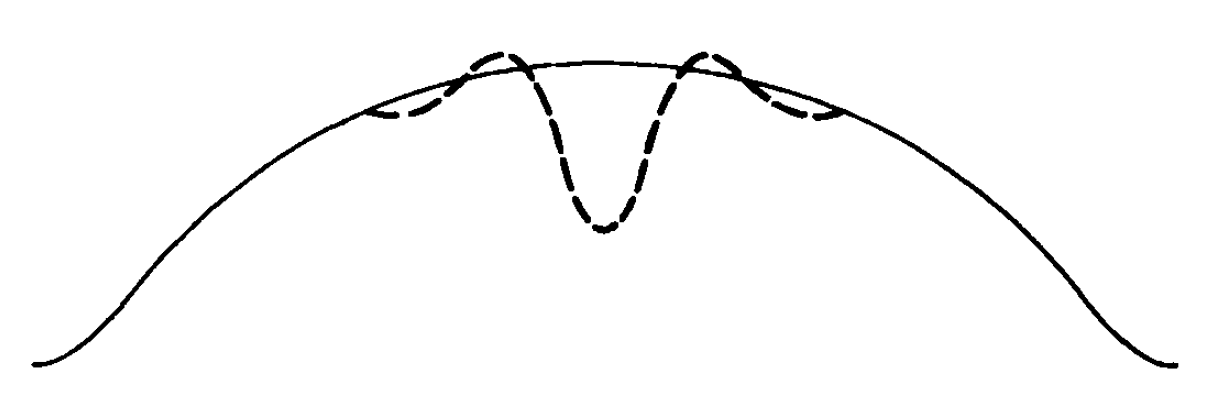
\includegraphics[width=\textwidth]{Figures/spurious}
        \caption[Point-source response (broken line) removal at the maximum of a broad feature, Clark (1982)]{Point-source response (broken line) removal at the maximum of a broad feature, Clark (1982)~\citep[Pg.~431,~Fig.~11.2]{thompson2008interferometry}}
		\label{fig:clarkSpu}
\end{figure}

The negative sidelobes of the beam add new maxima, which are selected in subsequent cycles, and thus there is a tendency for the component subtraction points to be located at intervals equal to the spacing of the first sidelobe of the synthesised (dirty) beam. The resulting map contains a lumpy artifact introduced by CLEAN, but the map is consistent with the measured visibility data. Cornwell (1983) has introduced a modification of the CLEAN algorithm that is intended to reduce this unwanted modulation. The original CLEAN algorithm minimizes 
\begin{equation}
\sum_{i}w_i|V^{meas}_{i} - V^{model}_{i}|^2
\end{equation}where $V^{meas}_{i}$ the measured visibility at $(u_i, v_i)$, $w_i$ is the applied weighting, and $V^{model}_{i}$ the corresponding visibility of the CLEAN-derived model. The summation is taken over the points with nonzero data in the input transformation for the dirty map. Cornwell's algorithm minimizes 

\begin{equation}
\sum_{i}w_i|V^{meas}_{i} - V^{model}_{i}|^2 -\kappa{s}
\end{equation}

where $s$ is a measure of smoothness and $\kappa$, is an adjustable parameter. Cornwell finds that the mean-squared intensity of the model, taken with a negative sign, is an effective implementation of $s$.

The effects of visibility tapering appear in both the original map and the beam, and thus the magnitudes and positions of the components subtracted in the CLEAN process should be largely independent of the taper. However, since tapering reduces the resolution, it is a common practice to use uniform visibility weighting for maps that are processed using CLEAN. Alternatively, in difficult cases such as those involving extended, smooth structure, reduction of sidelobes by tapering may improve the performance of CLEAN.

In 1980, Clark introduced an important reduction in the computation required for CLEAN. This is based on subtraction of the point-source responses in the $(u ,v)$ plane and using the FFT for moving data between the $(u,v)$ and $(l, m)$ domains. The procedure consists of minor and major cycles. A series of minor cycles is used to locate the components to be removed by performing approximate subtractions using only a small patch of the synthesised dirty beam that includes the main beam and the major sidelobes. Then in a major cycle the identified point-source responses are subtracted, without approximation, in the $(u, v)$ plane. That is, the convolution of the delta functions with the dirty beam is performed by multiplying their Fourier transforms. The series of minor and major cycles is then repeated until the required stop condition is reached. Clark devised this technique for use with data from the VLA(Very Large Array (Radiotelescope)) and found that it reduced the computation by a factor of two to ten compared with the original CLEAN algorithm.

To summarize the characteristics of CLEAN, we note that it is simple to understand from a qualitative viewpoint and straightforward to implement, and that its usefulness is well proven. On the other hand, a full analysis of its response is difficult. The response of CLEAN is not unique, and it can produce spurious artifacts. It is sometimes used in conjunction with model-fitting techniques; for example, a disk model can be removed from the image of a planet and the residual intensity processed by CLEAN~(\citet[Pg. 432]{thompson2008interferometry}).
